\documentclass[border=10pt]{standalone}
\usepackage[svgnames]{xcolor}
\usepackage{amsmath}
\usepackage{pgfplots}
\pgfplotsset{compat=newest}
\usepackage[sfdefault]{FiraSans}
\usepackage{FiraMono}
\renewcommand*\familydefault{\sfdefault}
\begin{document}
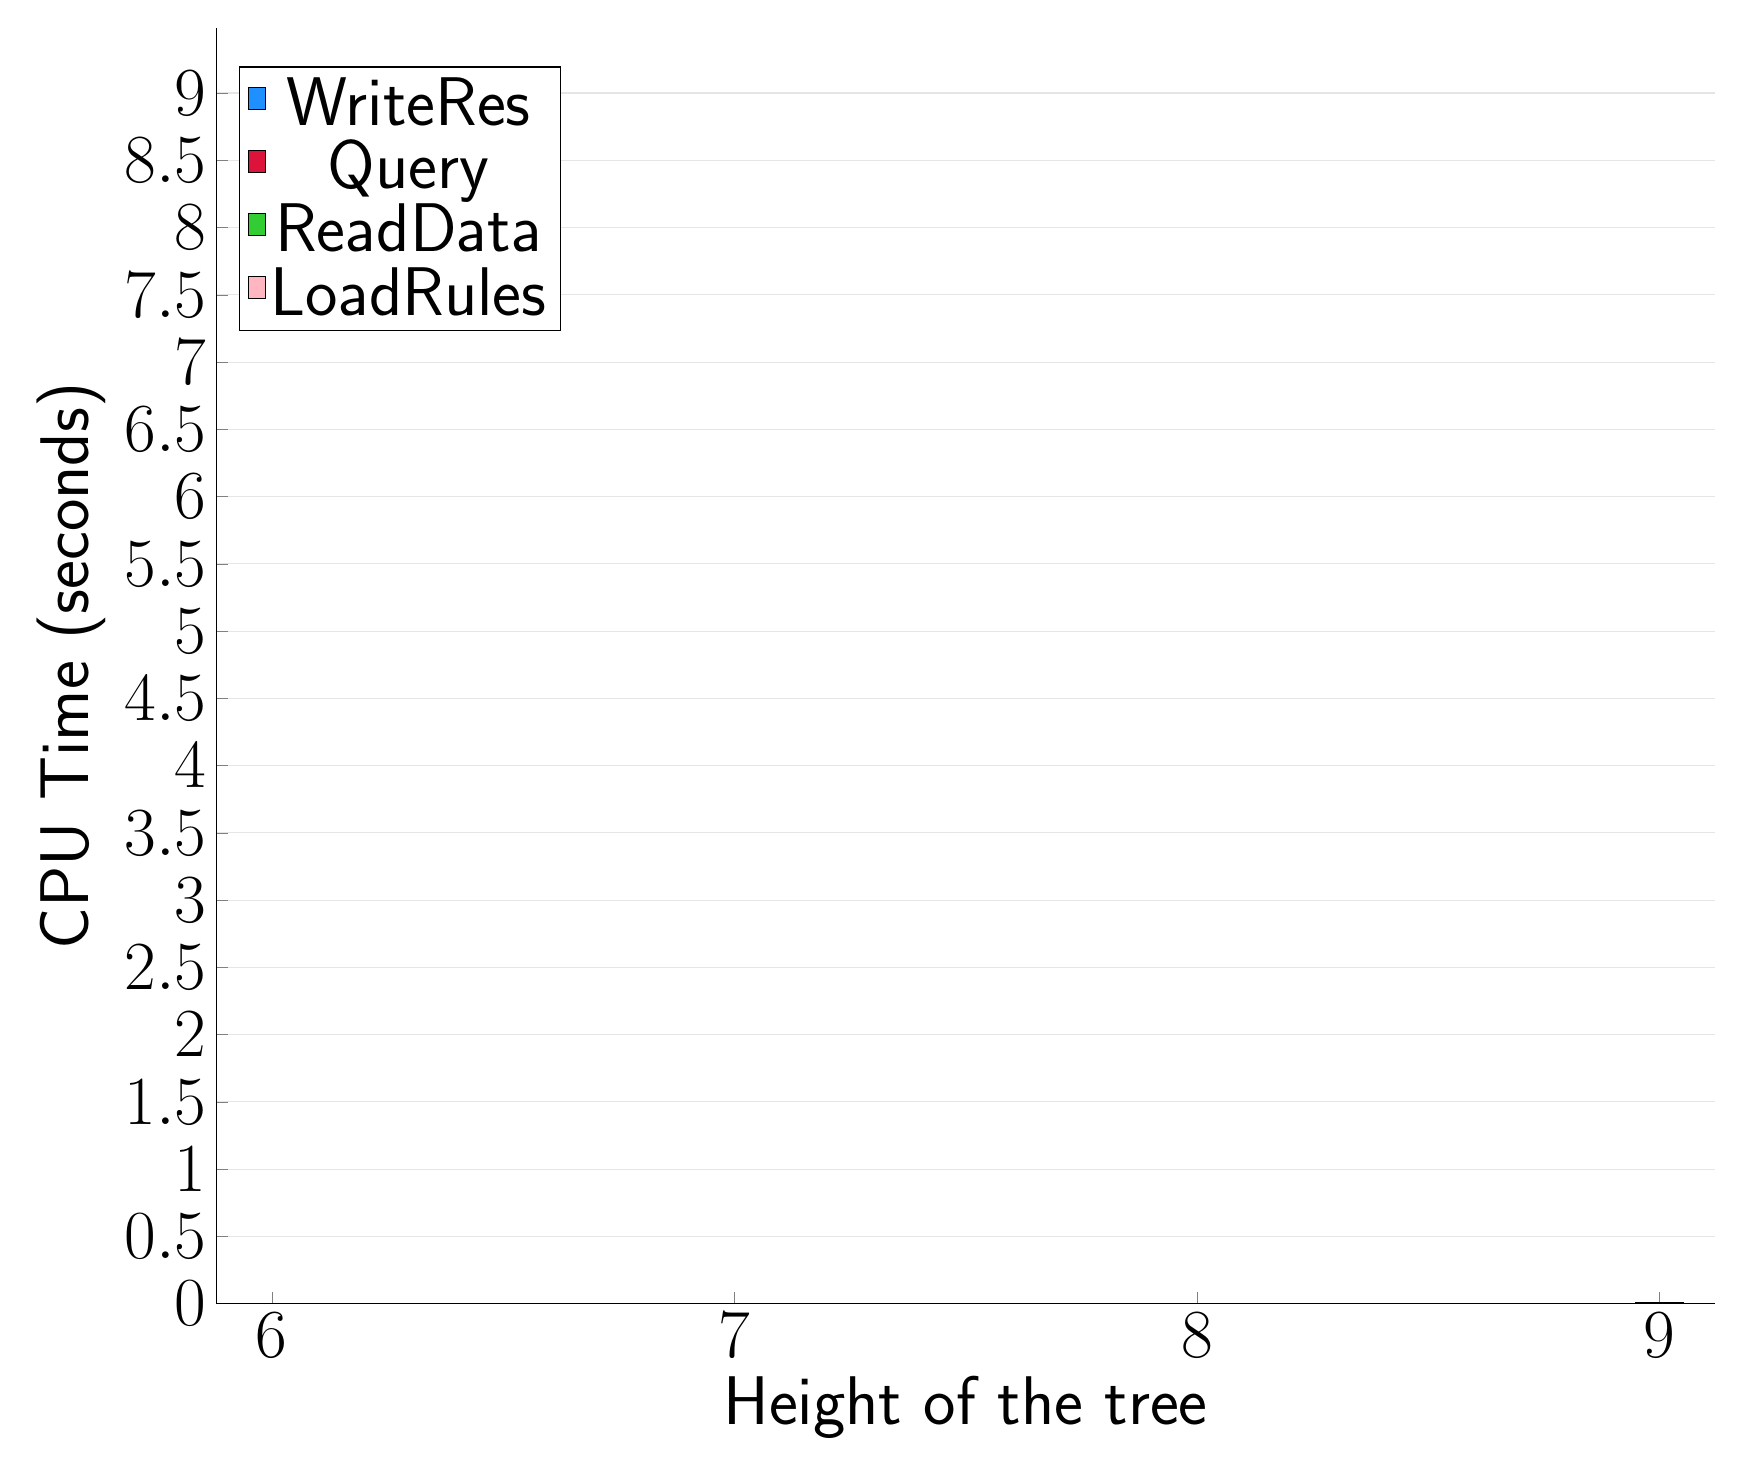
\begin{tikzpicture}
\begin{axis}[
   ybar stacked,
   width=1.7\textwidth,
   bar width=0.6cm,
   ymajorgrids, tick align=inside,
   major grid style={draw=gray!20},
   xtick=data,
   ymin=0, ymax=9.482,
   axis x line*=bottom,
   axis y line*=left,
   enlarge x limits=0.04,
   legend style={
       at={(0.23, 0.97)},
       anchor=north east,
       legend columns=1,
       font=\Huge,
   },
   ylabel={CPU Time (seconds)},
   xlabel={Height of the tree},
   label style={font=\Huge},
   tick label style={font=\Huge},
]
\addlegendimage{fill=DodgerBlue, draw=black, line width=0.2pt}
\addlegendentry{WriteRes}
\addlegendimage{fill=Crimson, draw=black, line width=0.2pt}
\addlegendentry{Query}
\addlegendimage{fill=LimeGreen, draw=black, line width=0.2pt}
\addlegendentry{ReadData}
\addlegendimage{fill=LightPink, draw=black, line width=0.2pt}
\addlegendentry{LoadRules}
\addplot +[fill=LightPink, draw=black, line width=0.55pt] coordinates {
(6, 0.0005478)
(7, 0.0005550000000000002)
(8, 0.0005485999999999999)
(8, 0.0005480000000000001)
(8, 0.0005479999999999997)
(9, 0.0005493999999999998)
(9, 0.0005548000000000003)
(9, 0.0005485999999999999)
(9, 0.0005449999999999997)
(9, 0.000545800000000001)
};
\addplot +[fill=LimeGreen, draw=black, line width=0.55pt] coordinates {
(6, 0.0001684000000000002)
(7, 0.00021859999999999978)
(8, 0.0003172000000000004)
(8, 0.0003174000000000002)
(8, 0.0003154000000000004)
(9, 0.0005192000000000006)
(9, 0.0005154000000000001)
(9, 0.0005182000000000001)
(9, 0.0005202000000000008)
(9, 0.0005162000000000001)
};
\addplot +[fill=Crimson, draw=black, line width=0.55pt] coordinates {
(6, 3.6400000000000004e-05)
(7, 7.679999999999978e-05)
(8, 0.0001719999999999998)
(8, 0.00017459999999999983)
(8, 0.0001704000000000004)
(9, 0.0004033999999999996)
(9, 0.0004075999999999998)
(9, 0.00040639999999999963)
(9, 0.000404)
(9, 0.0004073999999999996)
};
\addplot +[fill=DodgerBlue, draw=black, line width=0.55pt] coordinates {
(6, 0.00027759999999999965)
(7, 0.0006100000000000002)
(8, 0.0013488000000000003)
(8, 0.0013496)
(8, 0.0013515999999999995)
(9, 0.003065600000000001)
(9, 0.0030352)
(9, 0.0030496000000000004)
(9, 0.0030642)
(9, 0.0030372000000000003)
};
\end{axis}
\end{tikzpicture}

\end{document}
